\documentclass[12pt, twoside]{article}
\usepackage[francais]{babel}
\usepackage[T1]{fontenc}
\usepackage[latin1]{inputenc}
\usepackage[left=5mm, right=5mm, top=3mm, bottom=3mm]{geometry}
\usepackage{float}
\usepackage{graphicx}
\usepackage{array}
\usepackage{multirow}
\usepackage{amsmath,amssymb,mathrsfs}
\usepackage{textcomp}
\pagestyle{empty}
\usepackage{soul}

\begin{document} 


\begin{flushleft}
NOM PRENOM: \ldots \ldots \ldots \ldots \ldots \ldots \ldots \ldots \ldots
 \end{flushleft}


\begin{center}
{\fbox{$4^{e}3$ \qquad \qquad \textbf{\Large{Devoir surveill� 4}}
\qquad \qquad 08/02/2011}}
\end{center}


 
\enskip

\ul{\textbf{Exercice 1:}} \textit{(3,5 points)} Pour cet exercice, on ne
demande pas de justification.

\begin{tabular}{ccc}
\begin{minipage}{6cm}
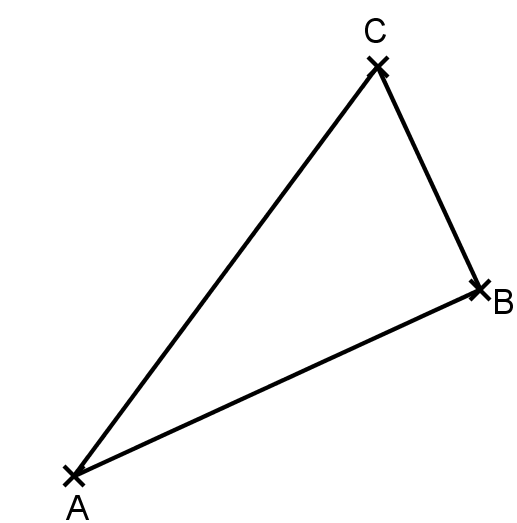
\includegraphics[width=35mm]{images/ex11.png}


\end{minipage}
&
\begin{minipage}{6cm}
\begin{center}
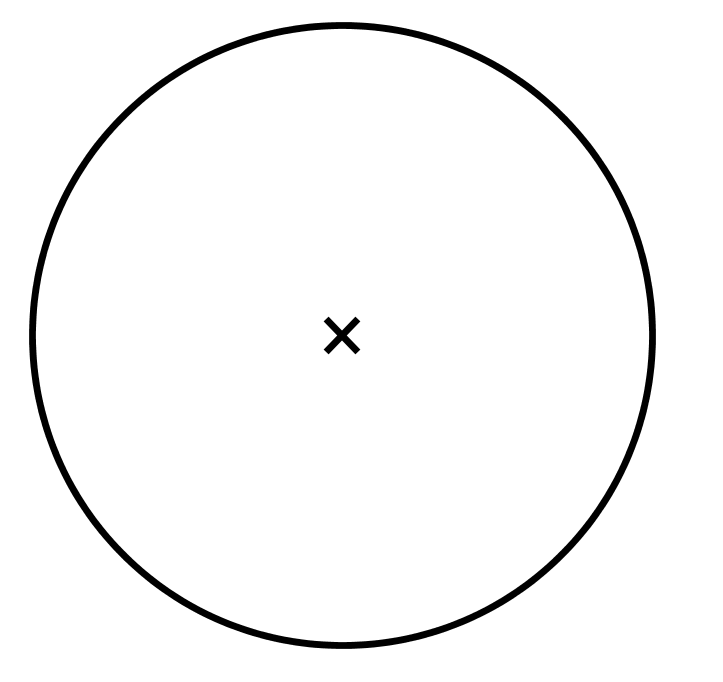
\includegraphics[width=35mm]{images/ex12.png}
\end{center}

\end{minipage}
&
\begin{minipage}{6cm}
\begin{center}
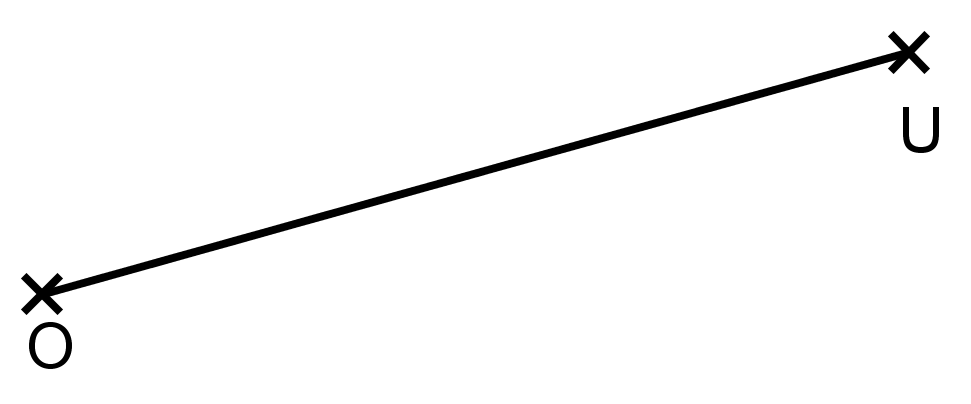
\includegraphics[width=35mm]{images/ex13.png}
\end{center}


\end{minipage} \\

\begin{minipage}{6cm}
1. Construire le cercle circonscrit 

au triangle ABC.
\end{minipage}
&
\begin{minipage}{6cm}
2. Construire un triangle DEF 

inscrit dans le cercle rectangle 

en D.
\end{minipage}
&
\begin{minipage}{6cm}
3. Construire un triangle OUI 

rectangle en I tel que UI=3cm.
\end{minipage}
\end{tabular}

 

\bigskip

\ul{\textbf{Exercice 2:}} \textit{(3 points)}


\begin{tabular}{cc}
\begin{minipage}{9cm}

En utilisant les informations port�es sur la figure:


\begin{enumerate}
  \item Calculer MN. Justifier votre r�ponse.
  \item En d�duire BC. Justifier votre r�ponse.
\end{enumerate}  
\end{minipage}
&
\begin{minipage}{9cm}
\begin{center}
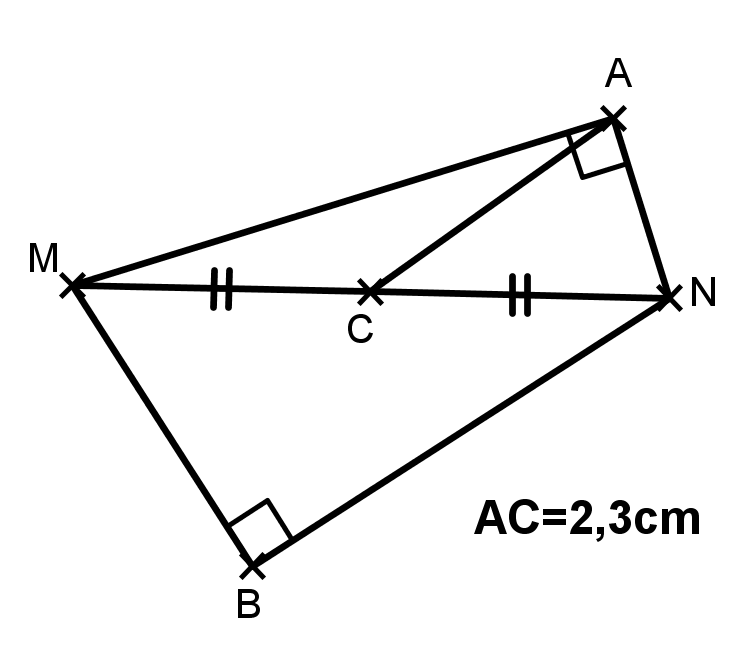
\includegraphics[width=40mm]{images/ex2.png}
\end{center}

\end{minipage}
\end{tabular}

\bigskip

\ul{\textbf{Exercice 3:}} \textit{(4,5 points)}




\begin{tabular}{cc}
\begin{minipage}{13cm}
Le segment [AI] est un diam�tre du cercle $\mathcal{C}_3$. 
E est un point de $\mathcal{C}_3$. 


Le cercle $\mathcal{C}_2$ a pour diam�tre [EI]. 
Le cercle $\mathcal{C}_1$ a pour diam�tre [AE]. 


Le point O est le point d'intersection des cercles $\mathcal{C}_1$ et
$\mathcal{C}_2$.

\begin{enumerate}
  \item Que peut-on dire du triangle AEI? Justifier votre r�ponse.
  \item Que peut-on dire du triangle AEO? Justifier votre r�ponse.
  \item Que peut-on dire du triangle EIO? Justifier votre r�ponse.
\end{enumerate}
 
\end{minipage}
&
\begin{minipage}{5cm}
\begin{center}
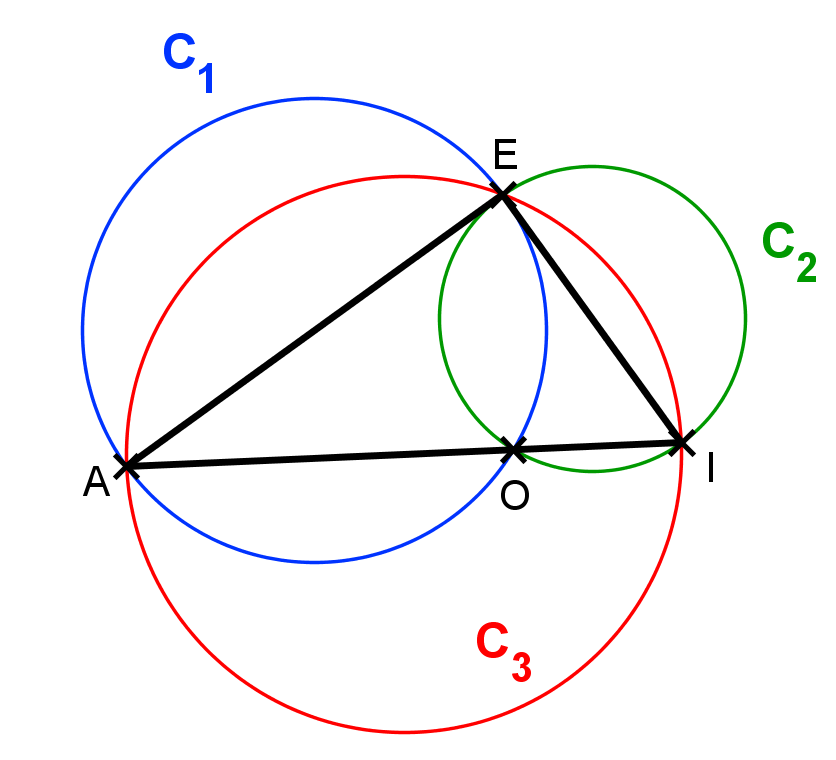
\includegraphics[width=5cm]{images/ex3.png}
\end{center}
\end{minipage}
\end{tabular}


\bigskip

\ul{\textbf{Exercice 4:}} \textit{(4 points)}

\begin{tabular}{cc}
\begin{minipage}{135mm}
\begin{enumerate}
  \item Montrer que le triangle AEC est rectangle en C. Justifier.
  \item Montrer que le point C est le milieu de [AM]. Justifie.
  \item Calculer AC.
  \item Calculer ED. Justifier votre r�ponse. 
\end{enumerate}
\end{minipage}
&
\begin{minipage}{55mm}
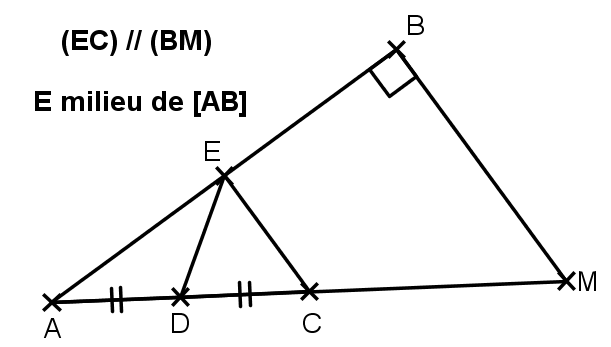
\includegraphics[width=55mm]{images/ex4.png}
\end{minipage}
\end{tabular} 

\bigskip 

\ul{\textbf{Exercice 5:}} \textit{(3,5 points)}

\quad



Un automobiliste a roul� sur l'autoroute � 120 km/h pendant 1h30min. Puis il
fait une pause d�jeuner. Il reprend la route et parcourt 250 km en 2h30min.

\begin{enumerate}
  \item Combien de kilom�tres a-t-il parcouru sur la premi�re partie du trajet?
  \item Quelle est sa vitesse moyenne pour la deuxi�me partie de son trajet?
  \item Quelle est sa vitesse moyenne sur l'ensemble de son trajet? 
\end{enumerate}

\bigskip

\ul{\textbf{Exercice 6:}} \textit{(1,5 points)}


Une antilope court � une vitesse de 24,5 m/s, un lion � une vitesse de 80 km/h.
Quel est le plus rapide de ces deux animaux? Justifier votre r�ponse.






\end{document}
